\documentclass{article}
\usepackage[top=1.25in, bottom=1in, left=1.25in, right=1.5in]{geometry}

\usepackage{graphicx}
\usepackage{float}

\begin{document}
\title{Milestone 1: Component Evaluation and Selection}
\author{Robert Amelard and Alexander Wong}
\maketitle

\noindent The first milestone from the CHI Project Plan document was to ``assist Hill-Rom in identifying a low cost camera module that is sensitive enough in the near infrared range, and that would enable pulse rate (PR) and respiratory rate (RR) monitoring through CHI''. This report presents the recommendations based on component evaluation and mutual discussion for a prototype device.

\section{Recommendations}
\subsection{Camera Module}
Driven primarily by NIR quantum efficiency and cost efficiency, the See3CAM\_CU30 (and e-CAM30\_CUMI0330\_MOD (3.4MP)) camera from e-con Systems was provided by Hill-Rom. The SeeCAM30\_CU30 integrates the 1/3'' ON Semi AR0330 sensor, which has 2.2~$\mu$m pixel pitch. Though the datasheet states it has full HD support at 60~fps, the iSpy software could only achieve 30~fps. Acquiring 60~fps (17~ms sampling interval) video is desirable to provide increased data sampling along the blood pulse waveform, but 30~fps (33~ms sampling interval) may be adequate for this application. Assuming a typical 100~ms blood pulse waveform rise time duration, 60~fps and 30~fps results in 6 and 3 discrete samples along the waveform, respectively. The sensor's quantum efficiency curve is shown below:

\begin{figure}[H]
\centering
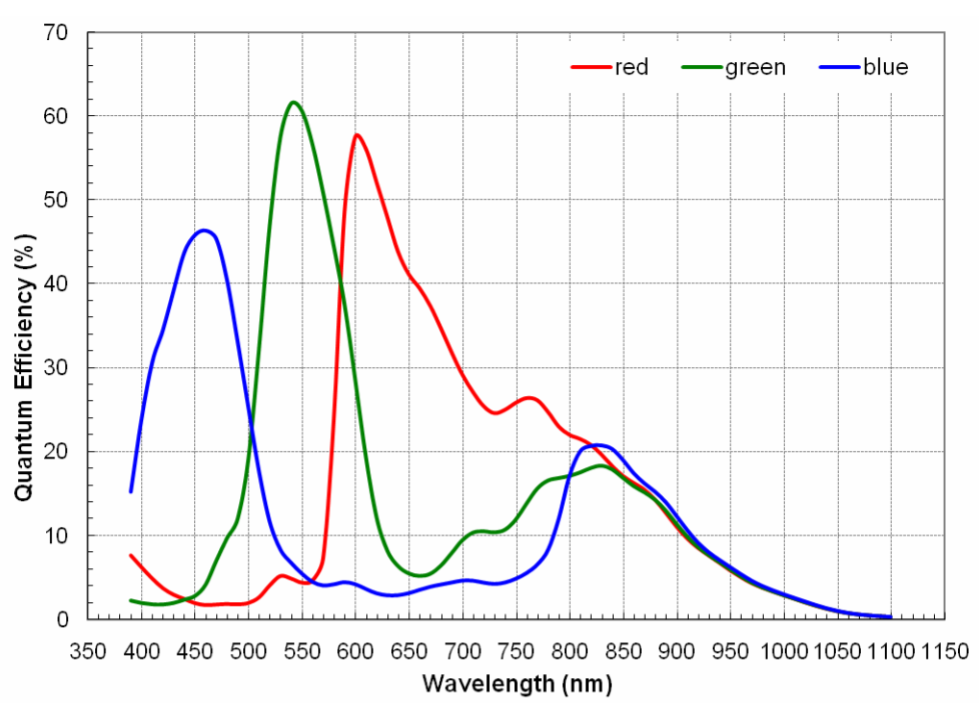
\includegraphics[width=0.7\textwidth]{QE}
\caption{Spectral quantum efficiency of the AR0330 sensor.}
\end{figure}

Though the camera integrates a Bayer filter grid, the three channels attain approximately the same QE at 850~nm (approx. 18\%). This is half as efficient as other sensors on the market, but it was determined that this camera should be used to integrate with Hill-Rom's existing embedded equipment. For a slight performance boost, the blue channel should be used for evaluation, which attains 1--2\% higher QE than the green and red channels.

The SeeCAM30 uses the S-mount lens mount, which was designed for small form factor. This reduced aperture size can be compensated by increasing the illumination output. However, in the future, if reduced power output is desired, a larger lens mount (e.g., C-mount, CS-mount) should be considered.

\subsection{Lighting Equipment}
The LEDEngin LZ4-00R608 was provided by Hill-Rom for evaluation. Upon evaluating the sensor readings, this component was deemed unnecessarily strong (and potentially hazardous if operated at the required 7~ft distance). Instead, the LEDEngin LZ1-LZ1-10R400 (850~nm) LED was chosen. This LED balances good radiant output with lower electrical requirements. A condensor lens and custom spatial homogenizer were placed in the illumination path to provide uniform and targeted irradiance.

As the intended use is long-term continuous monitoring in a clinical environment, the stability of the LED must be considered during design. A constant current driver for high-powered LEDs is recommended to power the LED, which stabilizes the current (and thus radiance) output of the LED by compensating for electrical and temperature fluctuations. We selected the TI LM3414HV constant current buck driver, which provides superior stability (max 1~A). This was evaluated using TI's LM3414HVMREVAL evaluation board.

\subsection{Optical Components}
Though many optical components could help reduce unwanted illumination variation, it was concluded that the number of optical components should be minimized to provide a cost efficient prototype system. Thus, several promising optical components were not evaluated for the scope of this project.

A NIR bandpass filter was acquired from MidOpt to eliminate stray ambient illumination on the sensor. This is an important optical component to develop a system that is agnostic to varying environmental conditions.

%Two NIR linear polarizers were considered for eliminating cutaneous specular reflectance (``glare''), but were deemed too costly for the system by Hill-Rom. These were therefore not evaluated.

\subsection{Camera Location}
Based on mutual discussion, the camera position will be constrained to overhead bed viewing at a distance of 7--9~ft (approx. 2--3~m). The face and neck should be easily viewed, with minimal shadow from overhead illumination. The optimal camera position is over the torso area, angled to view the neck and facial regions. All future evaluation protocols should adhere to this specification.

\section{Evaluation and Results}
Three evaluation procedures were performed to evaluate the different system characteristics: (1) camera noise, (2) pulsatility evaluation, (3) respiration evaluation. These results were used in the recommendations listed above. The details are described below.
%\subsection{Camera Noise}
%The camera was evaluated in a controlled environment to quantify its noise characteristics. [!!]

\subsection{Pulsatility Evaluation}
Pulsatility evaluation was conducted at two distances in a seated position. iSpy was used to record video. The NIR illumination provided 720~mW of optical power. CHI was used to evaluate the functional base case. CHI and the SeeCAM30 were integrated into a single system for spatially aligned frame acquisition. This is shown in the Figure~\ref{fig:setup}.

\begin{figure}[H]
\centering
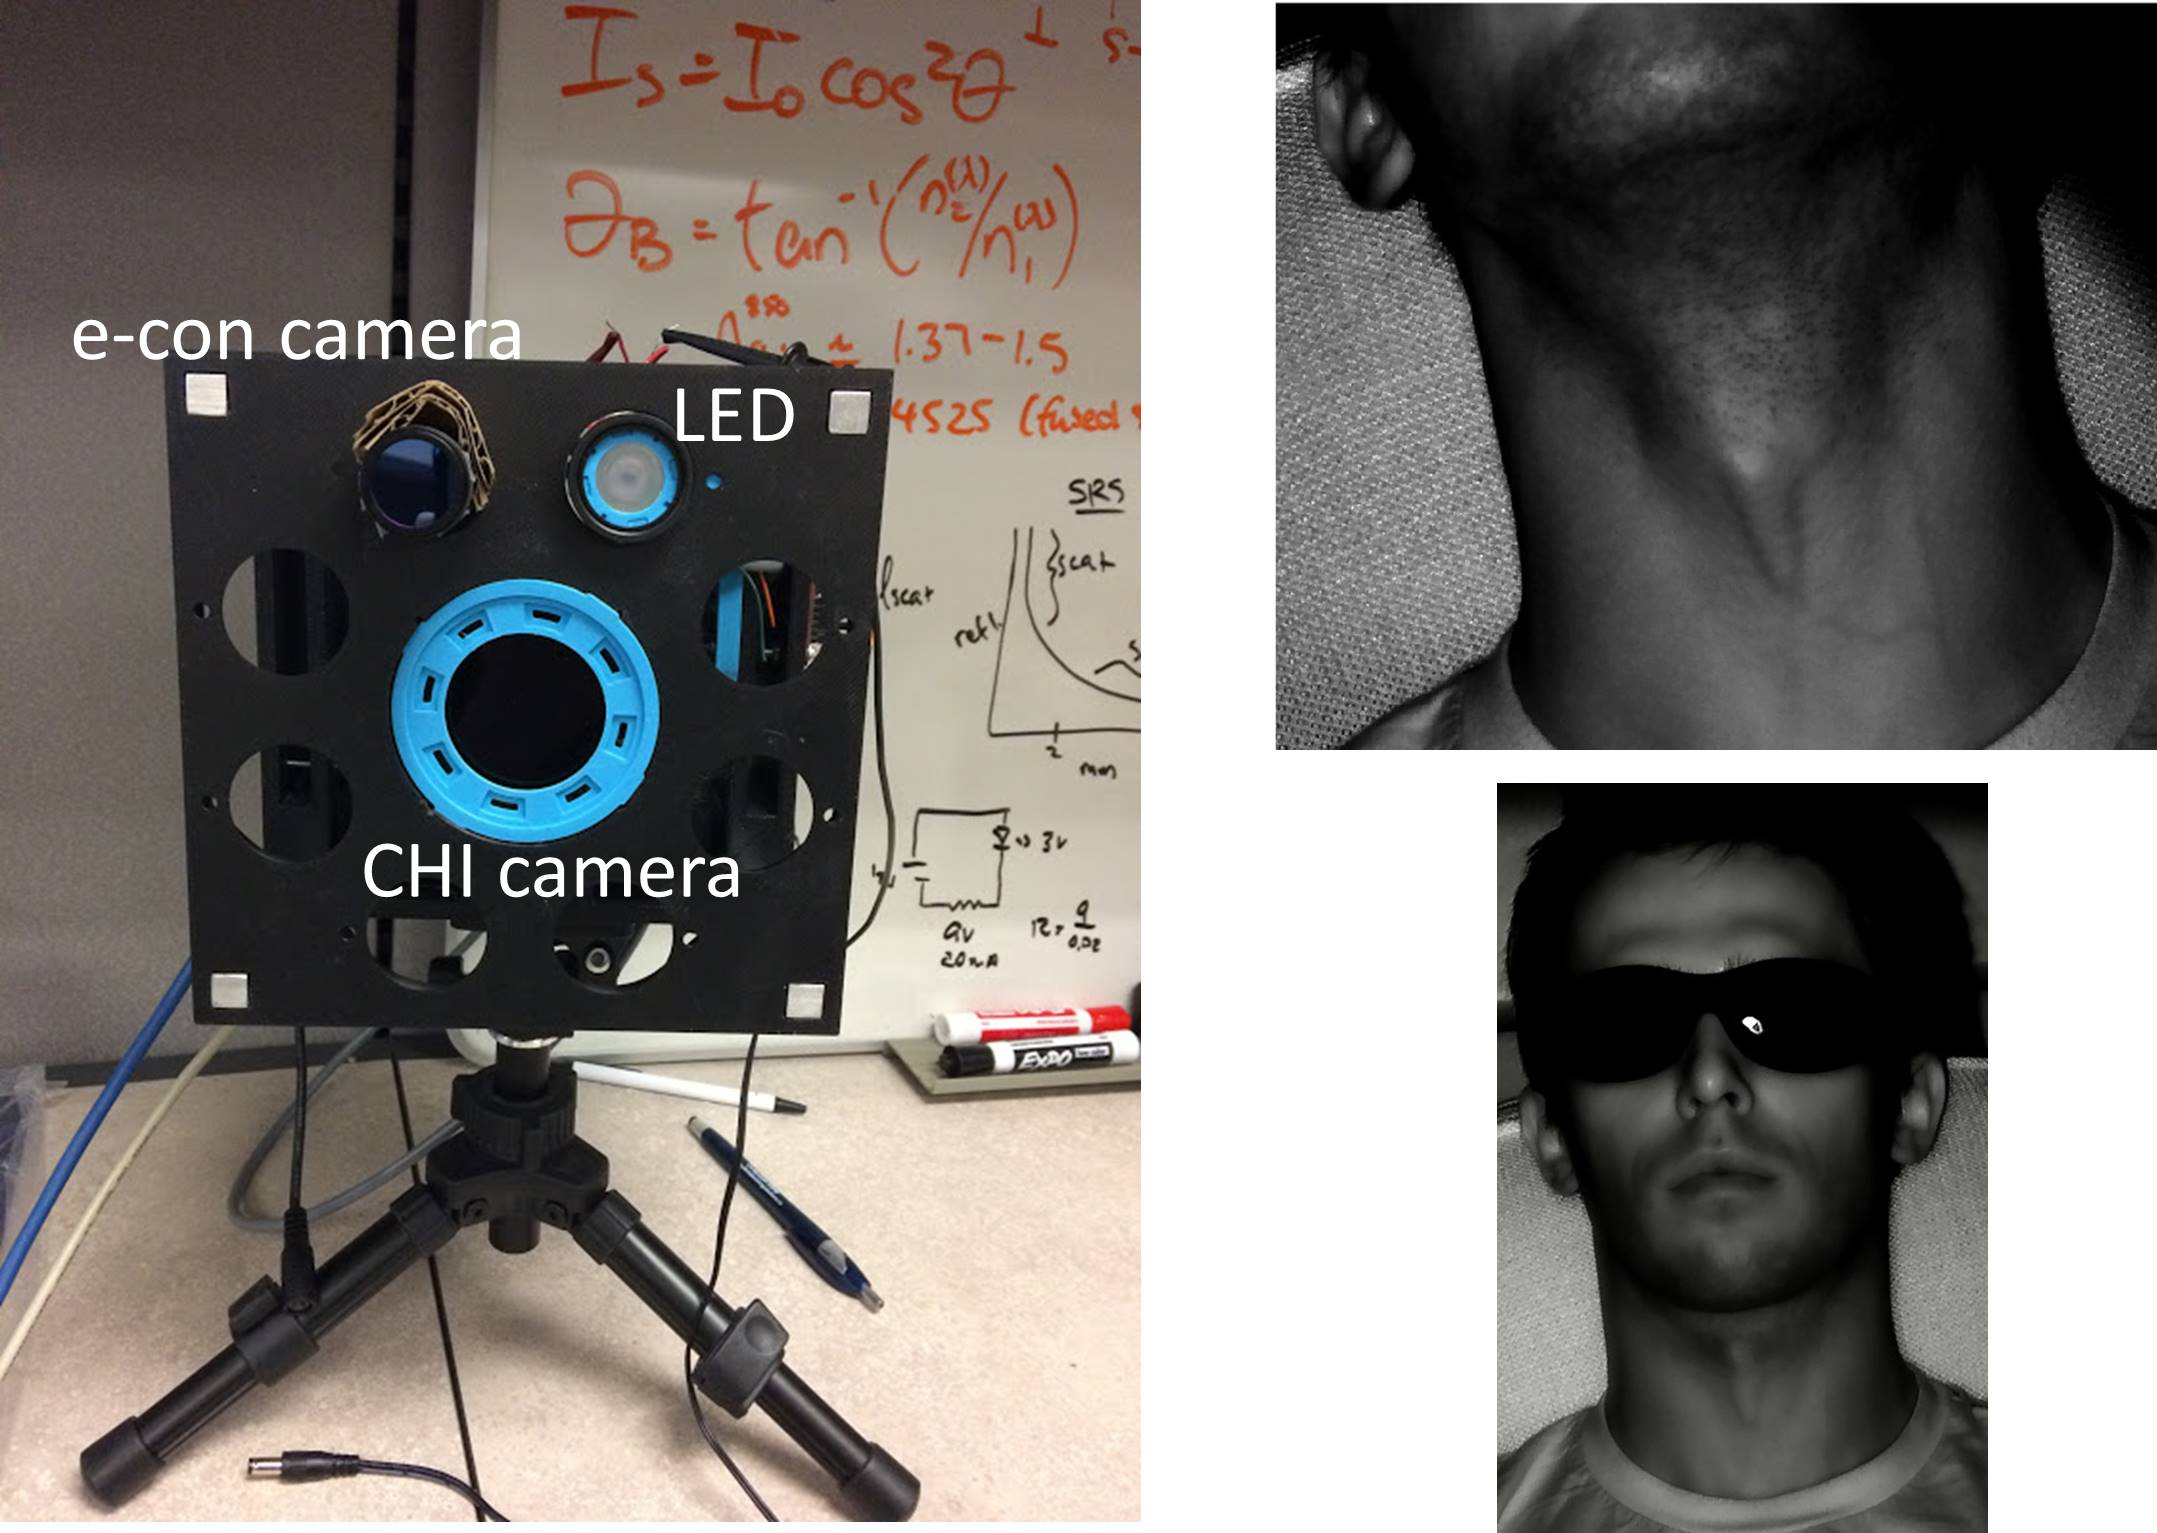
\includegraphics[width=0.5\textwidth]{setup}
\caption{Evaluation setup and sample frames.}
\label{fig:setup}
\end{figure}

\begin{figure}[H]
\centering
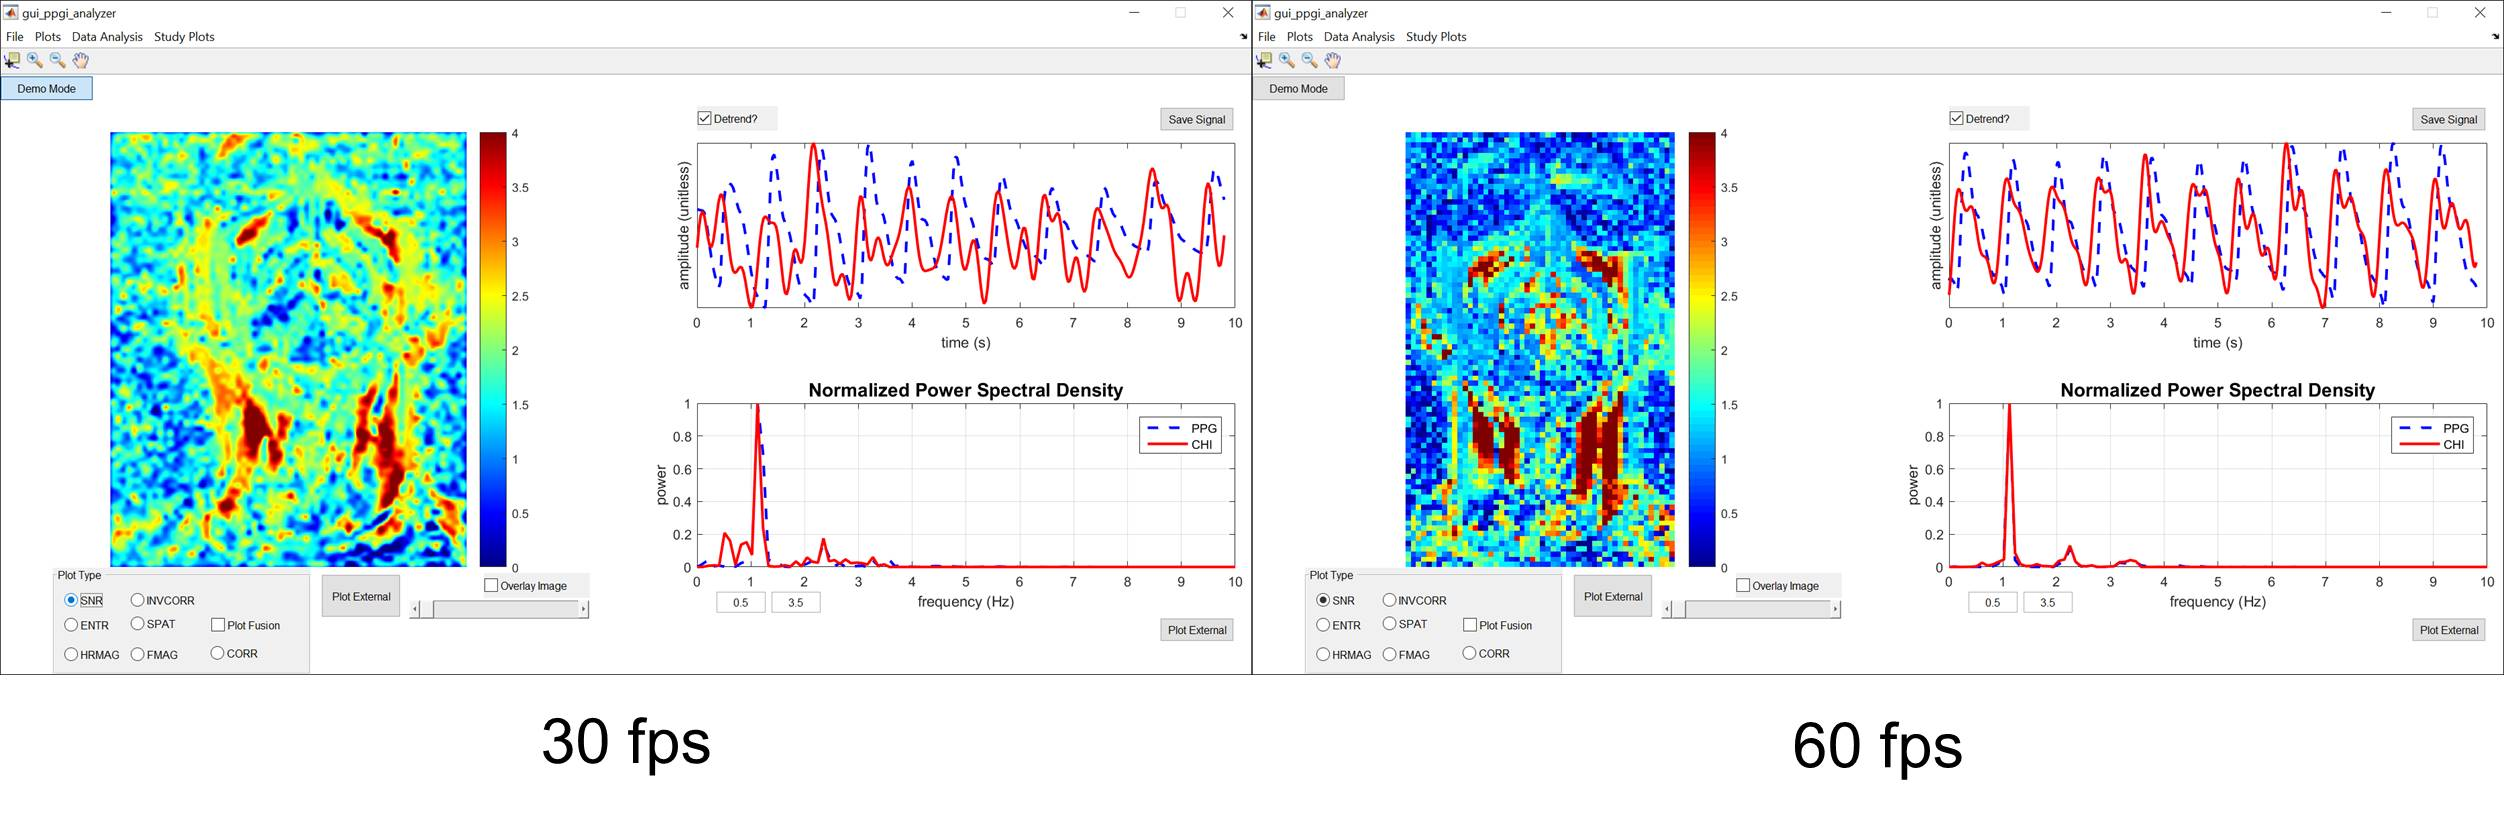
\includegraphics[width=\textwidth]{chi}
\caption{CHI was able to provide baseline results, showing strong pulsing up the neck through the cheeks. Notice that 60~fps video capture was able to provide significantly a better pulsatility signal than 30~fps, which is the maximum attainable frame rate of the SeeCAM30 in iSpy. 60~fps is preferred. This is discussed more below.}
\end{figure}

\begin{figure}[H]
\centering
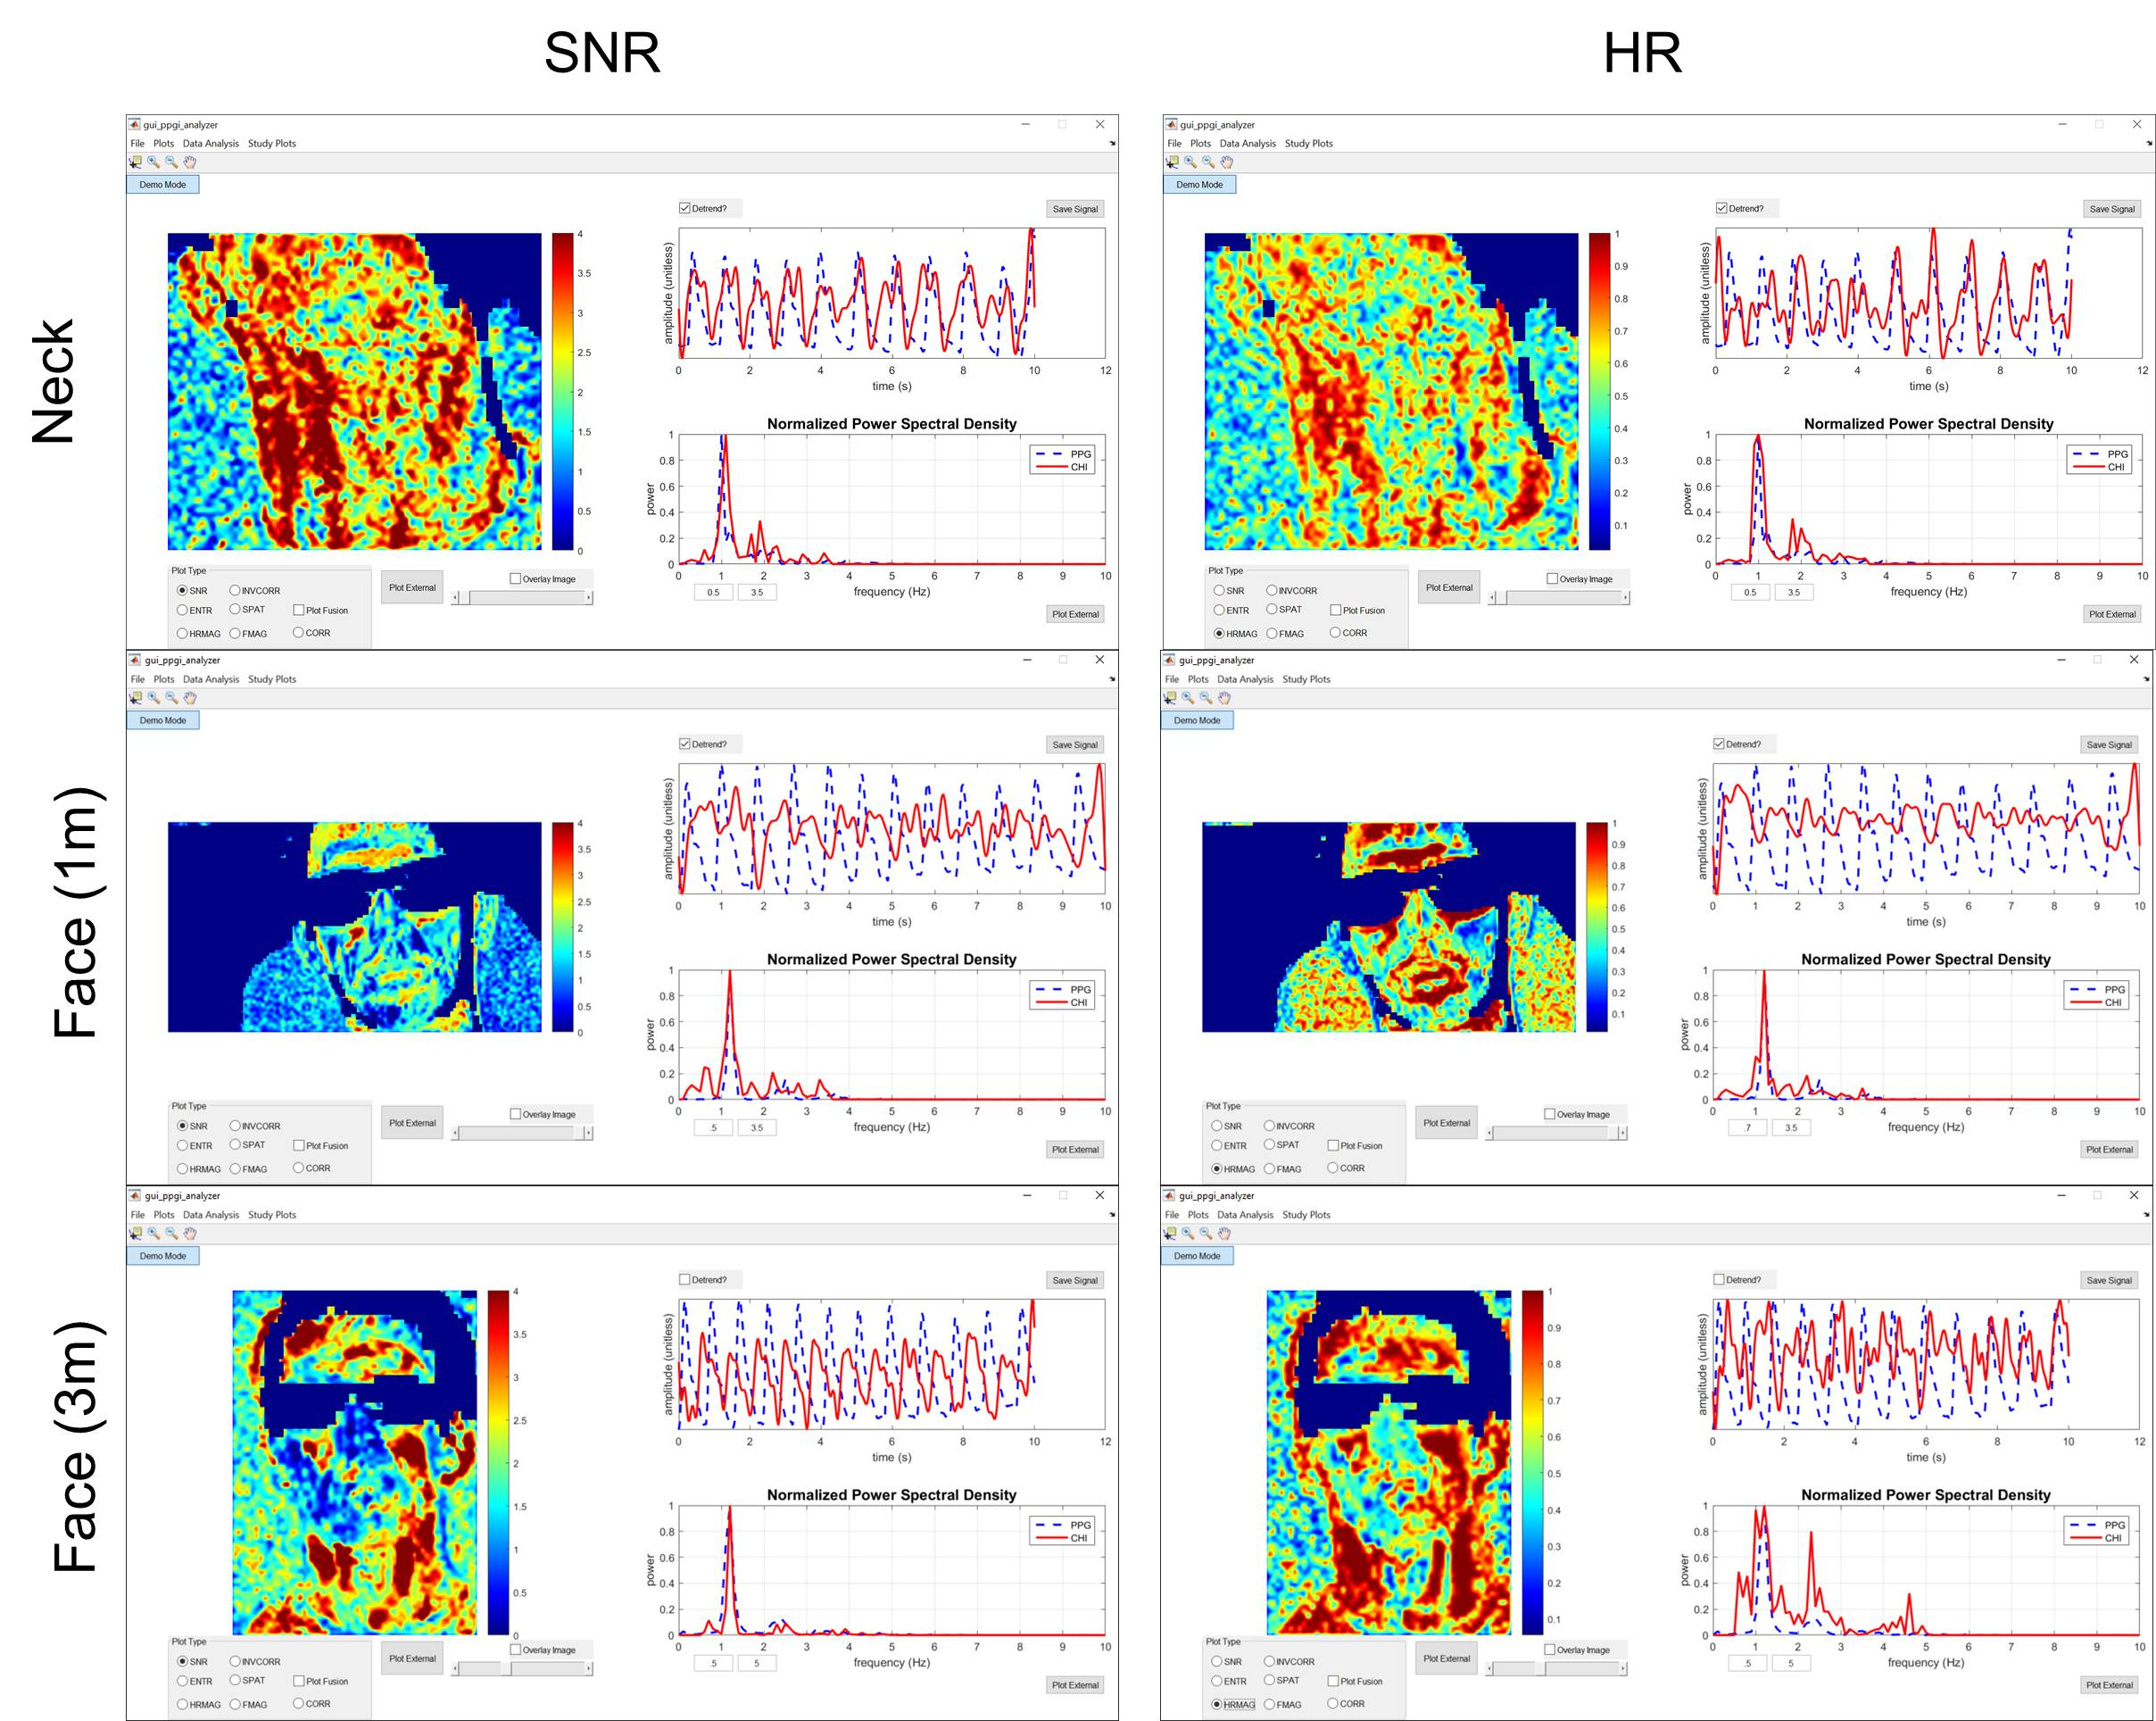
\includegraphics[width=\textwidth]{trials}
\caption{Evaluation trial grid, showing the maps of signal-to-noise ratio strength (SNR) and areas where heart rate was extracted (HR) at 1~m and 3~m distance (approx. 3~ft and 10~ft). Trials were conducted in a seated position. Pulsatility was observed in all trials (along the carotid track in the neck, and in the forehead and cheek area of the face), and heart rate could be extracted in the pulsatile locations. The 30~fps frame rate made it difficult during some trials to extract a clean blood pulse waveform due to sampling issues.}
\end{figure}

\subsection{Respiration Evaluation}
Similar to the method of respiratory inductance plethysmography bands, the volumetric effects of pulmonary ventilation can be measured by the mechanical movement of the chest and abdominal wall. Local pixel cohesion can be analyzed to measure volumetric disturbances from respiration. This is a promising technique given the target bed environment. This could potentially be augmented using concurrently acquired pressure sensor readings and/or thermal videos. An example of the results is shown below.

\begin{figure}[H]
\centering
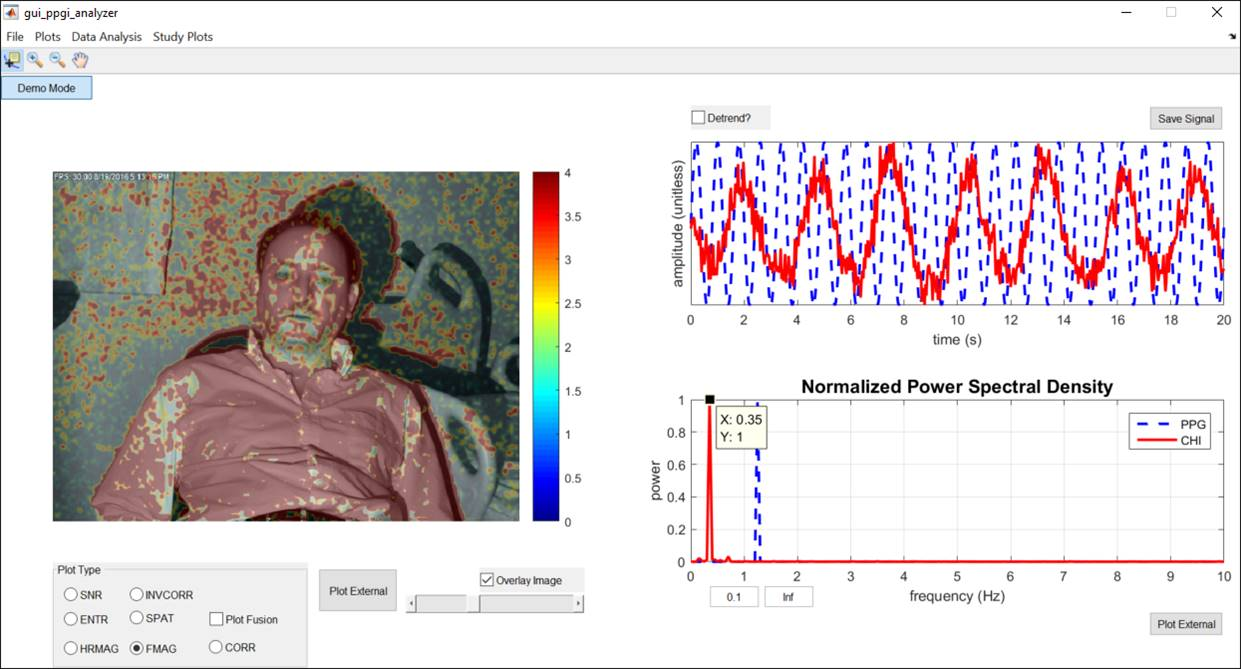
\includegraphics[width=0.7\textwidth]{respiration}
\caption{Respiration evaluation. Local volumetric disturbances from pulmonary ventilation were analyzed to extract the ventilation waveform (red) and rate (22~breaths per minute). The pixels highlighted in red indicate where the respiration waveform was extracted.}
\end{figure}


\section{Next Steps}
The current imaging system setup shows promise for strong cardiovascular pulsatility extraction from the required 7--9~ft distance. The next steps will be to use modify the imaging setup to collect data from overhead, simulating a hospital bed environment. Pilot data will be collected in this configuration and analyzed. Until the thermal camera module is functional, the facial region will be found using the imaging data for analysis. Automatic pulse rate and respiratory rate analysis will be analyzed. Upon availability, the thermal camera will be integrated into the system for guided facial segmentation.

\end{document}